\chapter{Implementation and Experiments}
\label{cp:implementation}
\label{cp:exp}
The propagator outlined in Chapter ~\ref{cp:AMOSUM} has been implemented in the ASP solver \textsc{wasp}
~\cite{DBLP:conf/lpnmr/AlvianoDLR15} using its Python interface ~\cite{DBLP:journals/tplp/DodaroR20}.
This design choice is motivated by the intuitive interface and its 
seamless integration with the solver through command-line options.
In our implementation, AMOSUM constraints are represented by facts, 
which are interpreted by the Python propagator. Specifically, the representation of an 
AMOSUM constraint $\sigma$ of the form (\ref{eq:amosum}) is the following:
\begin{align*}
\begin{array}{rr}
    \mathit{group}(\ell_i, w_i, g_i, \sigma) \leftarrow & \qquad\qquad \mathit{for\ all\ } i \in [1..n]\\
    \mathit{lb}(b, \sigma) \leftarrow
\end{array}
\end{align*}
where $\mathit{group}$ and $\mathit{lb}$ are reserved predicates.
Continuing Example~\ref{ex:amosum:propagation:more-2}, $\sigma_4$ is represented as follows:
\begin{align*}
\begin{array}{rr}
    \mathit{group}(x, 1, 1, \sigma_4) \leftarrow \\
    \mathit{group}(y, 2, 1, \sigma_4) \leftarrow \\
    \mathit{group}(z, 2, 2, \sigma_4) \leftarrow \\
    \mathit{group}(w, 3, 2, \sigma_4) \leftarrow \\
    \mathit{lb}(3, \sigma_4) \leftarrow 
\end{array}
\end{align*}

Moreover, since \textsc{wasp} already supports efficient propagators for handling AMO constraints, 
the Python propagator focuses on other inference rules, namely \eqref{eq:amosum:propagation:2} and \eqref{eq:amosum:propagation:3}, 
as described in Section~\ref{sec:amo:propagator}. Specifically, the \textit{propagate\_phase} function 
in~\ref{alg:propagate_phase} will not include the initial block for implementing the \textit{AMO inference rule}.
The \textit{AMO} constraint in \textsc{wasp} can be defined using a \textit{choice-rule} as follows:
\begin{align*}
    \{\ell_i : \group(\ell_i) = g\} \le 1 \leftarrow  \qquad\qquad \mathit{for\ all\ } g \in \mathbb{G}
\end{align*}

The implemented system, referred to as \textsc{amowasp}, was empirically assessed against the plain version 
of \textsc{wasp}~\cite{DBLP:conf/lpnmr/AlvianoDLR15} (version f3e4c56) and the state-of-the-art system \textsc{clingo} (version 5.4.0)~\cite{DBLP:conf/iclp/GebserKKOSW16}.
All the tested systems used \textsc{gringo} (included in the binary of \textsc{clingo}) as the grounder.

Experiments were conducted on an Intel Xeon 2.4 GHz server with 16 GB of memory.
There are three distinct modalities through which an experiment can be launched:
\begin{enumerate}
    \item No minimization of the reason (\textit{default}).
    \item Minimization of the reason (\textit{min}).
    \item Cardinality minimization of the reason (\textit{cmin}).
\end{enumerate}



\section{Benchmarks}

\paragraph{Synthetic Benchmark (SB).}%~\label{sec:synthetic}
Designed to empirically assess the intrisic properties of the AMO-SUM propagator.
The first benchmark comprises a program with a rule defining the set of groups $\mathbb{G}$ and another one incorporating a SUM aggregate.
The set $\mathbb{G}$ comprises 10 groups of uniform size $\mathit{group\_size} \in \{10, 100, 1000\}$, 
with the $i$-th literal of each group having weight $i$.
The bound of the SUM is set to
$\alpha \cdot C_1$ (achievable)
and
$C_1 + \alpha \cdot (C_2 - C_1)$ (unachievable), where:
$\alpha \in \{0.15, 0.45, 0.6, 0.9\}$;
$C_1$ is the sum of the maximum weight in each group, i.e., $10 \cdot \mathit{group\_size}$;
$C_2$ is the sum of all weights, i.e., $5 \cdot \mathit{group\_size} \cdot (\mathit{group\_size} + 1)$.
Hence, the benchmark comprises a total of 24 instances that are trivial for \textsc{amowasp} 
(they are solved without raising any conflict).
In contrast, \textsc{clingo} and \textsc{wasp} cannot perform the same inferences
and we have measured the number of conflicts found by the two systems within 
the first minute of computation.

\paragraph{Graph Coloring (GC).}%~\label{sec:hard}
The second benchmark is a modified version of the well-known Graph Coloring problem. 
In the Graph Coloring problem, the input consists of a graph and a set of colors, and the objective 
is to assign a color to each node so that connected nodes do not share the same color.
Here, colors are also associated with weights, and the sum of weights is required to reach a certain threshold value.
Instances are generated from those employed in the ASP competition~\cite{DBLP:journals/ai/CalimeriGMR16}, 
with the colors red, green, blue, yellow, and cyan associated with the weights 2, 4, 8, 16, and 64 to, respectively.
For each instance of $n$ nodes, the threshold is set to $\alpha \cdot 64 \cdot n$, where $\alpha \in \{0.15, 0.45, 0.75\}$.
This experiment aims to assess the performance of \textsc{amowasp} in comparison to two leading solvers, 
namely \textsc{clingo} and \textsc{wasp}, using real-world benchmarks. 
Time and memory were limited to 20 minutes and 15 GB, respectively.

\paragraph{Knapsack (K).}
A set of \emph{item types} is provided, each with an associated weight and value. 
Additionally, a knapsack capacity and a threshold are given. 
The objective is to determine whether it is possible to select a specific number of items 
from each type in such a way that the total weight remains within the knapsack capacity, 
while ensuring that the overall value reaches the specified threshold.
Instances were randomly generated as follows.
The number $n$ of types varies from $10$ to $55$ with an increasing step of 5.
The maximum number of items that can be selected for each type is fixed to $k = 20$.
The average value of the items is denoted as $v$ and used to define two critical thresholds:
$C_1 := n \cdot v \cdot k$ and $C_2 := n \cdot v \cdot (k \cdot (k+1)) / 2$. 
For each $n$, 10 instances are generated, categorized as follows:
(T1--T3) 3, 3 and 2 instances with a threshold sampled from a uniform distribution 
within the intervals [0, $C_1$], [0, $C_2$], and [$0.1 \cdot C_1$, $1.1 \cdot C_1$], respectively;
(T4) 2 instances with a threshold sampled from a normal distribution with a mean of $C_1$ and a variance of 5000.
Time and memory were limited to 20 minutes and 15 GB, respectively.

\section{Results}

\textbf{SB} has been tested only with the \textit{default} modality, 
whereas \textbf{KN} and \textbf{GC} have been tested with all three modalities:
\textit{default}, \textit{min}, and \textit{cmin}.
The experimental results for SB are summarized in Figure ~\ref{fig:resultssynthetic}. 
We can see that when $\mathit{group\_size}$ is 10 or 100, \textsc{clingo} can handle 
the first three instances in an efficient way, solving them with only a few conflicts. 
However, this is not true when $\mathit{group\_size}$ is $1000$. This suggests that the way 
in which \textsc{clingo} makes decisions (branching heuristic) works better for instances with 
SUM aggregates of small to medium size.
Moreover, as we expected, the number of conflicts is related to the bound. Specifically, 
instances with the smallest and largest bounds have fewer conflicts. 
This happens because these instances are either not constrained enough or overly constrained.


\begin{figure*}[h!]
    \centering
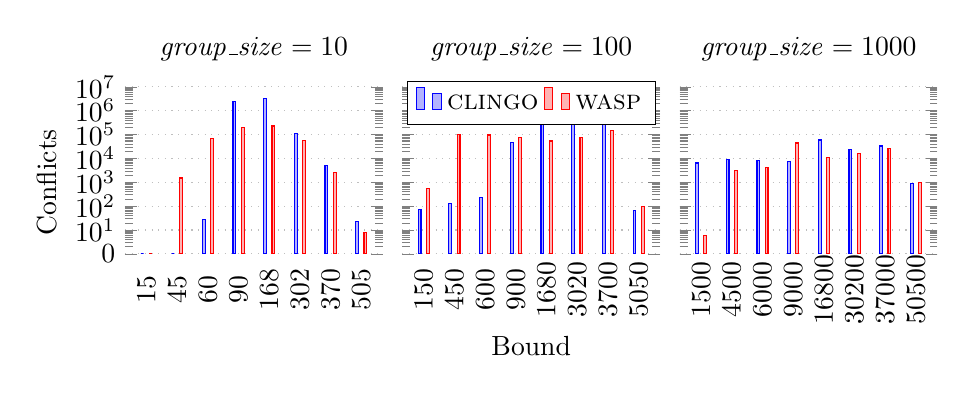
\begin{tikzpicture}
		\begin{axis}[
			xtick=data,
			xticklabels={$15$, $45$, $60$, $90$, $168$, $302$, $370$, $505$},
			ylabel={Conflicts},
            xlabel={},
            %xlabel={Asse x: bound/somma totale dei gruppi ($\mathit{bnd}_\sigma/\sum_{s \in S}{\max_{(w : \ell\ [s]) \in \sigma}w}$) per i diversi valori di $|\mathit{lits}_\sigma|_s|$},
            major x tick style=transparent,
			ybar,
			ymode=log,
			ymin=0.1,
			ymax=10000000,
			ytick={1, 10, 100, 1000, 10000, 100000, 1000000, 10000000},
			yticklabels={0, $10^1$, $10^2$, $10^3$, $10^4$, $10^5$, $10^6$, $10^7$},
			x axis line style={opacity=0},
            x tick label style={rotate=90, anchor=center},
			xtick=data,
			ymajorgrids=true,
			bar width=1pt,
			grid style=dotted,
			nodes near coords,
			scale only axis,
			point meta=explicit symbolic,
			% legend columns=-1,
			% legend pos=north east,
			height=0.2\textwidth,
			width=0.27\textwidth,
			name=plot1,
			title={$\mathit{group\_size} = 10$}
			]
			
			\addplot  coordinates {(0,1) (1,1) (2,27) (3, 2453921) (4, 3207378) (5, 112327) (6, 4845) (7, 22)};
            \addplot  coordinates {(0,1) (1,1506) (2,70594) (3, 194496) (4, 228698) (5, 58368) (6, 2492) (7, 8)};
			\legend{}
		\end{axis}	
		\begin{axis}[
			xtick=data,
			xticklabels={$150$, $450$, $600$, $900$, $1680$, $3020$, $3700$, $5050$},
			ylabel={},
            xlabel={Bound},
            %xlabel={Asse x: bound/somma totale dei gruppi ($\mathit{bnd}_\sigma/\sum_{s \in S}{\max_{(w : \ell\ [s]) \in \sigma}w}$) per i diversi valori di $|\mathit{lits}_\sigma|_s|$},
            major x tick style=transparent,
			ybar,
			ymode=log,
			ymin=0.1,
			ymax=10000000,
			ytick={1, 10, 100, 1000, 10000, 100000, 1000000, 10000000},
			yticklabels={},
			x axis line style={opacity=0},
            x tick label style={rotate=90, anchor=center},			
			xtick=data,
			ymajorgrids=true,
			bar width=1pt,
			grid style=dotted,
			nodes near coords,
			scale only axis,
			point meta=explicit symbolic,	
            legend columns=-1,
			% legend pos=north,
            legend style={at={(0.5,1.03)},anchor=north},
            height=0.2\textwidth,
			width=0.27\textwidth,
			name=plot2,
            at=(plot1.right of south east), anchor=left of south west,
			title={$\mathit{group\_size} = 100$}
			]
			
			\addplot  coordinates {(0,74) (1,124) (2,232) (3, 47209) (4, 263569) (5, 370134) (6, 476627) (7, 64)};
            \addplot  coordinates {(0,549) (1,100607) (2,95725) (3, 71962) (4, 53629) (5, 76733) (6, 152531) (7, 98)};	
            \legend{\textsc{clingo},\textsc{wasp}}
		\end{axis}
        \begin{axis}[
			xtick=data,
			xticklabels={$1500$, $4500$, $6000$, $9000$, $16800$, $30200$, $37000$, $50500$},
			ylabel={},
            xlabel={},
            %xlabel={Asse x: bound/somma totale dei gruppi ($\mathit{bnd}_\sigma/\sum_{s \in S}{\max_{(w : \ell\ [s]) \in \sigma}w}$) per i diversi valori di $|\mathit{lits}_\sigma|_s|$},
            major x tick style=transparent,
			ybar,
			ymode=log,
			ymin=0.1,
			ymax=10000000,
			ytick={1, 10, 100, 1000, 10000, 100000, 1000000, 10000000},
			yticklabels={},
			x axis line style={opacity=0},
			x tick label style={rotate=90, anchor=center},
			xtick=data,
            ymajorgrids=true,
			bar width=1pt,
			grid style=dotted,
			nodes near coords,
			scale only axis,
			point meta=explicit symbolic,            
			height=0.2\textwidth,
			width=0.27\textwidth,
			name=plot3,
            at=(plot2.right of south east), anchor=left of south west,
			title={$\mathit{group\_size} = 1000$}            
			]
			
			\addplot  coordinates {(0,6397) (1,8907) (2,8253) (3, 7461) (4, 59024) (5, 22660) (6, 33102) (7, 855)};
            \addplot  coordinates {(0,6) (1,3004) (2,4112) (3, 44378) (4, 10811) (5, 15519) (6, 25730) (7, 998)};									
		\end{axis}        
	\end{tikzpicture}
    \caption{
        Number of conflicts on synthetic AMOSUM constraints comprising 10 groups of varying size and bound.
        For each $\mathit{group\_size}$ there are four satisfiable instances (the first four bounds) and four unsatisfiable instances (the last four bounds).
        \textsc{amowasp} is not reported in the plots because it solves all tested instances in this benchmark without raising any conflict.
    }
    \label{fig:resultssynthetic}
\end{figure*}

The results obtained for GC and K are summarized in Figures~\ref{fig:graphcoloringknapsack}-~\ref{fig:scatter}.
As a first observation, \textsc{clingo} proves to be more efficient than \textsc{wasp} in both benchmarks.
As highlighted in SB, the branching heuristic of \textsc{clingo} is more effective than the one of \textsc{wasp}.
However, the inferences made by \textsc{amowasp} completely fulfil the gap related to the heuristic, and, in fact, \textsc{amowasp} achieves the best performance.
Regarding GC, \textsc{amowasp} successfully solves 72 instances, surpassing \textsc{clingo} and \textsc{wasp}, which solve 53 and 18 instances, respectively.
We additionally observe that the advantage of \textsc{amowasp} is particularly evident in instances with $\alpha = 0.75$, where it outperforms \textsc{clingo} and \textsc{wasp} by solving 48 and 60 more instances, respectively. However, for $\alpha = 0.15$ and $\alpha = 0.45$, the Python implementation introduces overhead, leading to comparatively poorer performance.
%
As for K, \textsc{amowasp} successfully solves 76 instances, outperforming both \textsc{clingo} and \textsc{wasp}, which solve 48 and 12 instances, respectively.
We additionally observe that \textsc{amowasp} consistently outperforms \textsc{wasp} across all instance categories,
solving 17, 25, 13, and 9 more instances of categories T1, T2, T3, and T4, respectively. 
In comparison to \textsc{clingo}, \textsc{amowasp} exhibits slightly poorer performance on T1 
instances, where \textsc{clingo} solves one more instance. However, 
it demonstrates better performance on the other instances, solving 16, 4, and 9 more T2, T3 and T4 instances, respectively.

\begin{figure*}[h]
    \begin{tikzpicture}[scale=0.7]
    \pgfkeys{%
        /pgf/number format/set thousands separator = {}}
    \begin{axis}[
    scale only axis
    , xlabel={Solved instances}
    , ylabel={Execution time (s)}
    , xmin=0, xmax=80
    , ymin=0, ymax=1220
    , legend style={at={(0.18,0.96)},anchor=north,fill=none}
    , legend columns=1
    , width=0.65\textwidth
    , height=0.40\textwidth
    , ytick={0,200,400,600,800,1000,1200}
    , major tick length=2pt
    , title= {Graph Coloring}
    ]
    \addplot [mark size=3pt, color=blue, mark=triangle*] [unbounded coords=jump] table[col sep=semicolon, y index=1] {./graphcoloringcactus.csv}; 
    \addlegendentry{\textsc{clingo}}
    
    \addplot [mark size=3pt, color=red, mark=triangle] [unbounded coords=jump] table[col sep=semicolon, y index=2] {./graphcoloringcactus.csv}; 
    \addlegendentry{\textsc{wasp}}
    
    \addplot [mark size=3pt, color=black, mark=o] [unbounded coords=jump] table[col sep=semicolon, y index=3] {./graphcoloringcactus.csv}; 
    \addlegendentry{\textsc{amowasp}}    
    \end{axis}
    \end{tikzpicture}%
    \hfill
    \begin{tikzpicture}[scale=0.7]
    \pgfkeys{%
        /pgf/number format/set thousands separator = {}}
    \begin{axis}[
    scale only axis
    , xlabel={Solved instances}
    , xmin=0, xmax=80
    , ymin=0, ymax=1220
    , legend style={at={(0.18,0.96)},anchor=north,fill=none}
    , legend columns=1
    , width=0.65\textwidth
    , height=0.40\textwidth
    , ytick={0,200,400,600,800,1000,1200}
    , yticklabels = {}
    , major tick length=2pt
    , title= {Knapsack}
    ]
    \addplot [mark size=3pt, color=blue, mark=triangle*] [unbounded coords=jump] table[col sep=semicolon, y index=1] {./knapsackcactus.csv}; 
    \addlegendentry{\textsc{clingo}}
    
    \addplot [mark size=3pt, color=red, mark=triangle] [unbounded coords=jump] table[col sep=semicolon, y index=2] {./knapsackcactus.csv}; 
    \addlegendentry{\textsc{wasp}}
    
    \addplot [mark size=3pt, color=black, mark=o] [unbounded coords=jump] table[col sep=semicolon, y index=3] {./knapsackcactus.csv}; 
    \addlegendentry{\textsc{amowasp}}    
    \end{axis}
    \end{tikzpicture}%
    \caption{
        Number of solved instances ($x$-axis) within a time limit ($y$-axis) for Graph Coloring (left) and Knapsack (right).
        %In particular, observe that \textsc{amowasp} solved XX and XX instances within 200 seconds of computation, while \textsc{wasp} and \textsc{clingo} only XX and XX, respectively.
    }\label{fig:graphcoloringknapsack}          
\end{figure*}


\begin{figure}
    \centering
\begin{tikzpicture}[scale=0.7]
    \pgfkeys{%
        /pgf/number format/set thousands separator = {}}
    \begin{axis}[
    scale only axis
    , legend style={at={(0.75,0.3)}, anchor=south, align=left}
    , legend cell align=left
    , xlabel={\textsc{wasp}}
    , ylabel={\textsc{amowasp}}
    , width=0.25\textwidth
    , height=0.25\textwidth
    , xmin=0, xmax=1200
    , ymin=0, ymax=1200
    , xtick={300,600,900,1200}
    , xticklabels={300,600,900,1200}
    , ytick={300,600,900,1200}
    , yticklabels={300,600,900,1200}
    , major tick length=2pt
    , title={Graph Coloring}
    ]
    \addplot [mark size=3pt, only marks, color=blue, mark=star] [unbounded coords=jump] table[col sep=semicolon, x index=4, y index=5] {graphcoloringscatter15.csv};     
    \addlegendentry{$\alpha = 0.15$}

    \addplot [mark size=3pt, only marks, color=darkorange, mark=o] [unbounded coords=jump] table[col sep=semicolon, x index=4, y index=5] {graphcoloringscatter45.csv};
    \addlegendentry{$\alpha = 0.45$}

    \addplot [mark size=3pt, only marks, color=darkgreen, mark=triangle] [unbounded coords=jump] table[col sep=semicolon, x index=4, y index=5] {graphcoloringscatter75.csv};     
    \addlegendentry{$\alpha = 0.75$}

    \addplot [color=red, dashed] [unbounded coords=jump] coordinates {(0,0) (1200,1200)}; 
    \end{axis}
\end{tikzpicture}
\begin{tikzpicture}[scale=0.7]
    \pgfkeys{%
        /pgf/number format/set thousands separator = {}}
    \begin{axis}[
    scale only axis
    , legend style={at={(0.75,0.3)}, anchor=south, align=left}
    , legend cell align=left
    , xlabel={\textsc{clingo}}
    %, ylabel={\textsc{amowasp}}
    , width=0.25\textwidth
    , height=0.25\textwidth
    , xmin=0, xmax=1200
    , ymin=0, ymax=1200
    , xtick={300,600,900,1200}
    , xticklabels={300,600,900,1200}
    , ytick={300,600,900,1200}
    , yticklabels={}
    , major tick length=2pt
    , title={Graph Coloring}
    ]
    \addplot [mark size=3pt, only marks, color=blue, mark=star] [unbounded coords=jump] table[col sep=semicolon, x index=3, y index=5] {graphcoloringscatter15.csv};     
    \addlegendentry{$\alpha = 0.15$}

    \addplot [mark size=3pt, only marks, color=darkorange, mark=o] [unbounded coords=jump] table[col sep=semicolon, x index=3, y index=5] {graphcoloringscatter45.csv};
    \addlegendentry{$\alpha = 0.45$}

    \addplot [mark size=3pt, only marks, color=darkgreen, mark=triangle] [unbounded coords=jump] table[col sep=semicolon, x index=3, y index=5] {graphcoloringscatter75.csv};     
    \addlegendentry{$\alpha = 0.75$}

    \addplot [color=red, dashed] [unbounded coords=jump] coordinates {(0,0) (1200,1200)}; 
    \end{axis}
\end{tikzpicture}


\begin{tikzpicture}[scale=0.7]
    \pgfkeys{%
        /pgf/number format/set thousands separator = {}}
    \begin{axis}[
    scale only axis
    , legend style={at={(0.75,0.3)}, anchor=south, align=left}
    , legend cell align=left
    , xlabel={\textsc{wasp}}
    , ylabel={\textsc{amowasp}}
    , width=0.25\textwidth
    , height=0.25\textwidth
    , xmin=0, xmax=1200
    , ymin=0, ymax=1200
    , xtick={300,600,900,1200}
    , xticklabels={300,600,900,1200}
    , ytick={300,600,900,1200}
    , yticklabels={300,600,900,1200}
    , major tick length=2pt
    , title={Knapsack}
    ]
    \addplot [mark size=3pt, only marks, color=blue, mark=star] [unbounded coords=jump] table[col sep=semicolon, x index=4, y index=5] {knapsackscatter-type1.csv};     
    \addlegendentry{T1}

    \addplot [mark size=3pt, only marks, color=darkorange, mark=o] [unbounded coords=jump] table[col sep=semicolon, x index=4, y index=5] {knapsackscatter-type2.csv};
    \addlegendentry{T2}

    \addplot [mark size=3pt, only marks, color=darkgreen, mark=triangle] [unbounded coords=jump] table[col sep=semicolon, x index=4, y index=5] {knapsackscatter-type3.csv};     
    \addlegendentry{T3}
    
    \addplot [mark size=3pt, only marks, color=darkviolet, mark=square] [unbounded coords=jump] table[col sep=semicolon, x index=4, y index=5] {knapsackscatter-type4.csv};     
    \addlegendentry{T4}

    \addplot [color=red, dashed] [unbounded coords=jump] coordinates {(0,0) (1200,1200)}; 
    \end{axis}
\end{tikzpicture}
\begin{tikzpicture}[scale=0.7]
    \pgfkeys{%
        /pgf/number format/set thousands separator = {}}
    \begin{axis}[
    scale only axis
    , legend style={at={(0.75,0.3)}, anchor=south, align=left}
    , legend cell align=left
    , xlabel={\textsc{clingo}}
    %, ylabel={\textsc{amowasp}}
    , width=0.25\textwidth
    , height=0.25\textwidth
    , xmin=0, xmax=1200
    , ymin=0, ymax=1200
    , xtick={300,600,900,1200}
    , xticklabels={300,600,900,1200}
    , ytick={300,600,900,1200}
    , yticklabels={}
    , major tick length=2pt
    , title={Knapsack}
    ]
    \addplot [mark size=3pt, only marks, color=blue, mark=star] [unbounded coords=jump] table[col sep=semicolon, x index=3, y index=5] {knapsackscatter-type1.csv};     
    \addlegendentry{T1}

    \addplot [mark size=3pt, only marks, color=darkorange, mark=o] [unbounded coords=jump] table[col sep=semicolon, x index=3, y index=5] {knapsackscatter-type2.csv};
    \addlegendentry{T2}

    \addplot [mark size=3pt, only marks, color=darkgreen, mark=triangle] [unbounded coords=jump] table[col sep=semicolon, x index=3, y index=5] {knapsackscatter-type3.csv};     
    \addlegendentry{T3}
    
    \addplot [mark size=3pt, only marks, color=darkviolet, mark=square] [unbounded coords=jump] table[col sep=semicolon, x index=3, y index=5] {knapsackscatter-type4.csv};     
    \addlegendentry{T4}

    \addplot [color=red, dashed] [unbounded coords=jump] coordinates {(0,0) (1200,1200)}; 
    \end{axis}
\end{tikzpicture}
    \caption{
        Instance-by-instance comparison on the execution time (in seconds) required to solve Graph Coloring and Knapsack.
        (Timeouts normalized to 1200 seconds.)
        Points below the red dashed line are instances in which \textsc{amowasp} is faster than the compared system.
    }\label{fig:scatter}
\end{figure}

To sum up, \textsc{amowasp} outperforms \textsc{wasp} thanks to the technique presented in this paper, 
as \textsc{amowasp} is powered by \textsc{wasp} and thus inherits all of its heuristic parameters.

